\subsection{SPMD at Nano-Scale}
\label{sec:modelling_nano}

%% 1. Introduction: How to get more variations
%% 2. How to generate the equations
%% 3. Explain Alignment how power monitor is aligned with event trace
%%    3a. Explain gradient method to align 
%% 4. Explain the results
%%    4a. Explain problems in CPU Base power
%%    4b. Explain problems in per-core CPU power
%%    4c. Explain problems in GPU
%% 5. Reasons for the equation not giving correct solution
%% 6. Conclusion

Given that the component usage diversity 
seems to mainly exist within each rendering interval yet creating two equations per interval
are not enough, we next explore setting up multiple model equations, each at an even finer scale, within each 16.7ms interval. We denote this approach as {\it SPMD at nano-scale}.

\paragraph{Methodology}
%% 2. How to generate the equations
The methodology is similar to that of micro-scale SPMD, except
that instead of generating two equation per 16.7 ms interval,
we generate 16 equations, \ie one equation for every 1ms sub-interval. 
We tried 1, 2, 4, and 8 number of 16.7 ms intervals and show results for 1 interval \ie 16 equations.
Due to page limit; the other results are very similar. 

\if 0
\begin{table}[tp]
{\footnotesize
    \centering
    \caption{Normalized vector distance between 16.7 ms intervals for nano-scale SPMD for Moto Z3.}
    \vspace{-0.1in}
    \begin{tabular}{|c|c|c|c|}
    \hline
        App & Scenario & Mean & Standard deviation \\
        \hline
         \multirow{2}{20mm}{Boat Racing} & Into & 0.00 & 0.07 \\
         \cline{2-4}
         & Still & 0.00 & 0.03 \\
         \hline
         \multirow{2}{20mm}{Bricks Breaker} & Into & 0.00 & 0.07 \\
         \cline{2-4}
         & Still & 0.00 & 0.03 \\
         \hline
        \multirow{2}{20mm}{Candy Crush Saga} & Into & -0.00 & 0.13 \\
        \cline{2-4}
	     & Tutorial & 0.00 & 0.05 \\
	     \hline
    \end{tabular}
    \label{tab:nano-distance}
    \vspace{-0.1in}
}
\end{table}
% From each the of the 16.7 ms interval we get 16 equations.

\paragraph{Fine-grained trace alignment}
For SPMD at nano-scale, the main challenge is to align the power and the data traces. 
Since we have 1ms sub-interval and the power monitor resolution is 0.2ms, it is critical to
align power draw readings of the power monitor with data collected on the phone.
We find that the method of generating a beacon using a CPU burst is too coarse-grained for this purpose. To achieve good alignment, we did two things. 
First, we observed in the power trace, there are sharp variations or gradient whenever the GPU state changes between Busy and Idle within each 16.7ms frame rendering interval. We therefore developed a technique to automatically identify the sharp
positive gradients in the power trace which corresponds to start of the GPU Busy state.
The Busy state and Idle state duration are obtained from the Linux event trace.

However, we may still not be able to align an interval in the power monitor reading with
the correct interval in the data collection. To overcome this,
we observe that the adjacent 16.7ms intervals
have very similar energy drain at 1ms resolution
and hence misalignment by one or more intervals will not affect the resulting equations significantly. 
% As a worst case, alignment algorithm can only introduce misaligment in multiple of 16.7 ms.
To see this, we represented the energy drain of each 16.7 ms interval by a 16-element vector, with each element corresponding to the energy drain of a 1ms interval.
% We find the normalized distance vector between two consecutive 16.7 ms intervals, $i^{th}$ and $i+1^{th}$
% by element wise subtracting and dividing it with their averages.
% We then calculated the normalized distance between two adjacent vectors as the average of the elements on normalized distance vector.
We then generated the normalized distance between the vectors 
for 60 consecutive 16.7 ms intervals.
The results are shown in Table~\ref{tab:nano-distance} for Moto Z3.
We observe the mean value for all four app scenarios 
to be 0.00 with standard deviation less than 0.13.
We conclude that the 16.7 ms interval is highly repetitive and robust to misalignment by a few multiples 16.7 ms.
% \comment{To align the event trace with the power trace,
% we first observe each start of the Active-busy state in the event trace,
% and then find the nearest power trace Active-busy peak to align each 16.7 ms duration.
% -- this does not seem enough-- what is the two traces are of by many multiples of the 16.7ms?}

% We ignore some of the cases where the algorithm is not converging enough.
\fi

\begin{figure*}[tp]
    \centering
     \begin{subfigure}[b]{0.32\textwidth}
         \centering
         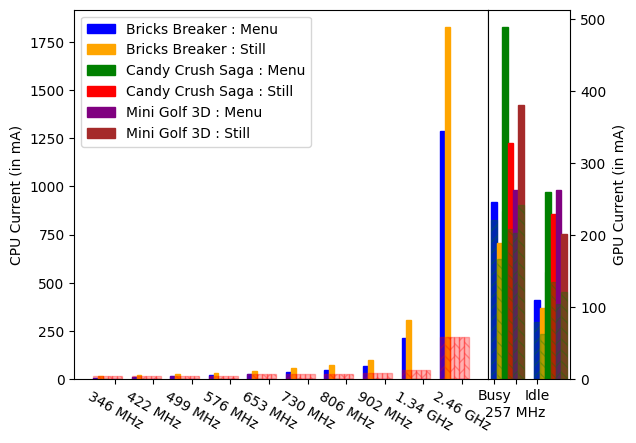
\includegraphics[width=\textwidth]{figures/002_Pixel2_1_nano_equations.png}
         \label{fig:number_parameters_vs_duration_100s_0}
     \end{subfigure}
    \begin{subfigure}[b]{0.32\textwidth}
         \centering
         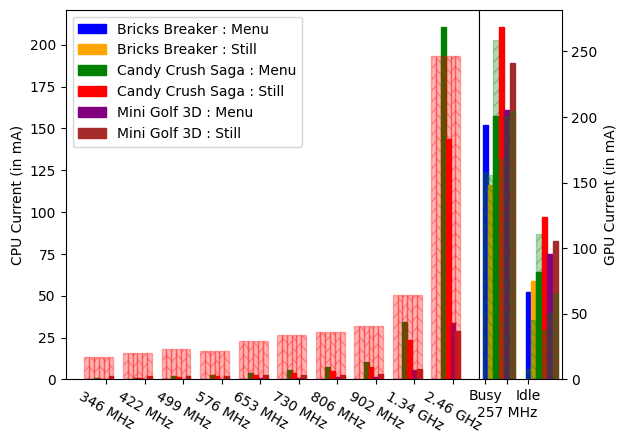
\includegraphics[width=\textwidth]{figures/003_MotoZ3_1_nano_equations.png}
         \label{fig:number_parameters_vs_duration_100s_100}
     \end{subfigure}
    \begin{subfigure}[b]{0.32\textwidth}
         \centering
         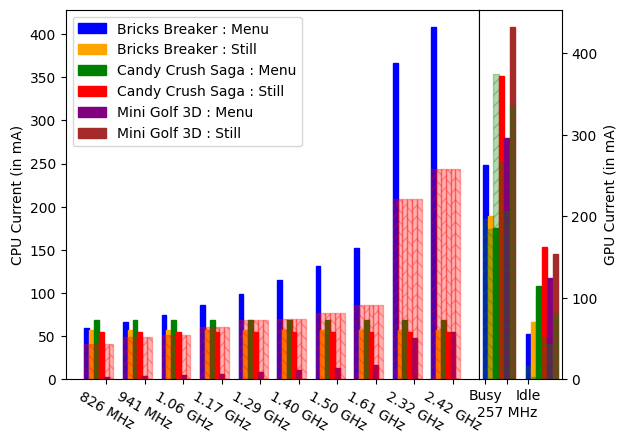
\includegraphics[width=\textwidth]{figures/004_Pixel4_1_nano_equations.png}
         \label{fig:number_parameters_vs_duration_100s_200}
     \end{subfigure}
     \hfill
     \centering
     \begin{subfigure}[b]{0.32\textwidth}
        \centering
    	{ \scriptsize
    	\begin{tabular}{ | l | c | c | c | c | c | c | }
    		\hline
    		     & \multicolumn{6}{ c|}{Error for each App Scenarios (in \%)}\\
    		\cline{2-7}
                    Model & \rot{B. Menu} & \rot{B. Still} & \rot{C. Menu} & \rot{C. Still} & \rot{M. Menu} & \rot{M. Still}  \\
    		\hline
                Fix. F. Const.       & 4.3 & 3.8 & 12 & 9.1 & 5.5 & 16 \\
                Classical            & 19 & 30 & 23 & 22 & 51 & 31 \\

    		\hline
    	\end{tabular}
    	}
	\caption{Pixel 2}
    \end{subfigure}
         \begin{subfigure}[b]{0.32\textwidth}
        \centering
    	{ \scriptsize
    	\begin{tabular}{ | l | c | c | c | c | c | c | }
    		\hline
    		     & \multicolumn{6}{ c|}{Error for each App Scenarios (in \%)}\\
    		\cline{2-7}
                    Model & \rot{B. Menu} & \rot{B. Still} & \rot{C. Menu} & \rot{C. Still} & \rot{M. Menu} & \rot{M. Still}  \\
    		\hline
                Fix. F. Const.       & 14 & 14 & 7.3 & 14 & 21 & 12 \\
                Classical            & 42 & 18 & 39 & 27 & 41 & 18 \\
    		\hline
    	\end{tabular}
    	}
	\caption{Moto Z3}
    \end{subfigure}
         \begin{subfigure}[b]{0.32\textwidth}
        \centering
    	{ \scriptsize
    	\begin{tabular}{ | l | c | c | c | c | c | c | }
    		\hline
    		     & \multicolumn{6}{ c|}{Error for each App Scenarios (in \%)}\\
    		\cline{2-7}
                    Model & \rot{B. Menu} & \rot{B. Still} & \rot{C. Menu} & \rot{C. Still} & \rot{M. Menu} & \rot{M. Still}  \\
    		\hline
                Fix. F. Const.       & 13 & 11 & 16 & 27 & 21 & 25 \\
                Classical            & 38 & 50 & 23 & 42 & 29 & 34 \\
    		\hline
    	\end{tabular}
    	}
	\caption{Pixel 4}
    \end{subfigure}
     \hfill
    \caption{Model parameters derived by nano-scale SPMD}
    \label{fig:nano}
    \vspace{-0.1in}
\end{figure*}

\paragraph{Findings}
Figure~\ref{fig:nano} shows the model parameters output of the Fixed Freq-constrained regression solver for the same six app scenarios.
We observe that the model parameters derived from nano-scale SPMD are again drastically different from the corresponding parameters derived from the classical model.
In particular, we see that for Moto Z3 for "Fix-Freq.-Constr. SPMD" for 16 equations
(1)The power models output by the solver have LSF error
between 6.4\% to 25.5\% for Pixel 2, between 4.3\% to 22.3\% for Moto Z3 and between 10.4\% to 33.9\% for Pixel 4
% (2) Depending upon The CPU model parameters are in the range of 0 mA ,0 mA,0-81 mA for Pixel 2 ,Moto Z3,Pixel 4 respectively.
(2)For  Pixel 4 out of 6 app scenarios CPU parameters are zero for 2 scenarios and less than 50\% of the classical model parameters for 3 scenarios .
Similarly, CPU parameters are zero for 2 scenarios and less than 50\%  of the classical model parameters for 4 scenarios for Moto Z3.
Whereas, CPU parameters are zero for Pixel 2.
% \comment{(2) In 3 out of the 12 scenarios marked in bold, the model parameters generated seem reasonable, \ie about 50\% of their counterparts in the classic model.}

\begin{table}[tp]
{\footnotesize
    \centering
    \caption{The rank and singular values for the set of equations for nano-scale "Fix-Freq.-Constr. SPMD" for Pixel 4  for 16 equation system of equation.
    (Top 4 singular values are shown.)
    }
    \vspace{-0.1in}
    \begin{tabular}{|c|p{9mm}|p{4.5mm}|p{4.5mm}|p{4.5mm}|p{4mm}|p{4mm}|p{4mm}|}
    \hline
        App & Scenario & Num. of Eqns. & Num. of Vars. & Rank &  \multicolumn{3}{c|}{Singular Values} \\
        \hline
        \multirow{2}{13mm}{Bricks Breaker} & Menu & 16 & 4 & 4 & 4.15  & 2.21  & 1.51 \\
         \cline{2-8}
         & Still & 16 & 4 & 4 & 4.16  & 1.65  & 1.11 \\
         \hline
        \multirow{2}{13mm}{Candy Crush Saga} & Menu & 16 & 4 & 4 & 4.34  & 3.00  & 2.28 \\
        \cline{2-8}
	     & Still & 16 & 4 & 4 & 4.86  & 2.69  & 0.87 \\
	     \hline
         \multirow{2}{13mm}{Mini Golf 3D} & Menu & 16 & 5 & 5 & 3.88  & 2.90  & 1.31 \\
         \cline{2-8}
         & Still & 16 & 5 & 5 & 4.14  & 3.10  & 2.18\\
         \hline

    \end{tabular}
    \label{tab:nano-rank_motoz3}
    \vspace{-0.1in}
}
\end{table}

Table~\ref{tab:nano-rank_motoz3} shows the systems of equations are full rank and have reasonable singular values for Moto Z3. 
%
% The rank is one off of the full rank due to the fact that CPU base power does not vary.
% To overcome this, we fixed the base power to the constant
% base power parameter value from the classical model, making the set of equations full rank.
% The model parameters output by the solver with this constraint 
% are shown in the rows labeled as "Fix-Freq-constr." in the same two tables.
% We observe that the solutions are still different from those in the classic
% model; in particular, the constraint simply shifted the high based power to high GPU Idle power.

\begin{table}[tp]
    \centering
    \caption{Equations for the 16.7 ms interval for Bricks Breaker Menu scenario on Moto Z3 for 16 equation set.}
    {\small
    \begin{tabular}{|c|c|c|c|c|}
        \hline
            Eqn & y(n) & \multicolumn{1}{c|}{CPU Utilization} & \multicolumn{2}{c|}{GPU Utilization} \\
%       \cline{2-4}
%            y(n)  & 422 MHz & \multicolumn{2}{c|}{257 MHz} \\
        \cline{4-5}
            & (mA) & \multicolumn{1}{c|}{} & Busy & Idle \\
        \hline
                 1 & 273.1 &  43\% &  100\% &    0\% \\
                 2 & 341.2 &   0\% &  100\% &    0\% \\
                 3 & 348.0 & 105\% &   78\% &   21\% \\
                 4 & 184.8 & 135\% &    0\% &  100\% \\
                 5 & 153.5 & 184\% &    0\% &  100\% \\
                 6 & 155.6 & 130\% &    0\% &  100\% \\
                 7 & 164.3 & 147\% &    0\% &  100\% \\
                 8 & 164.6 & 115\% &    0\% &  100\% \\
                 9 & 169.0 & 125\% &    0\% &  100\% \\
                10 & 166.7 & 127\% &    0\% &  100\% \\
                11 & 164.6 & 100\% &    0\% &  100\% \\
                12 & 166.8 & 124\% &    0\% &  100\% \\
                13 & 171.3 & 108\% &    0\% &  100\% \\
                14 & 166.2 & 137\% &    0\% &  100\% \\
                15 & 154.2 & 180\% &    0\% &  100\% \\
                16 & 165.7 & 124\% &    2\% &   97\% \\
        \hline
    \end{tabular}
    }
    \label{tab:equations_nano}
\end{table}

Finally, we looked into the individual equations to understand why 
Table~\ref{tab:equations_nano} shows the 16 equations for the 16.7 ms interval for Bricks Breaker Menu scenario for Moto Z3.
We make two observations.
(1) The equations fall into two groups, corresponding to the GPU Busy state and Idle state with equation corresponding to the transition. 
(2) Within each group, many equations contradict each other. For example,
the CPU utilization of Eqn.~14 are higher than 
those in Eqn.~13 yet the LHS energy values are the opposite. The same happens for group 2, \eg between Eqn.~1 and Eqn.~2. 
These numbers suggest that again the 16 equations not only did not add to the diversity, but actually
added noise to the equations making it hard for the solver to output meaningful model parameters. 

% \if 0
% We observe the some equation are not following the excepted trend.
% Like in $11^{th}$ and $12^{th}$ equations, the CPU utilization has gone up from 218\% to 328\% but the LHS fell from 160.00 mA to 153.20 mA.
% In nano-scale the measurement noise is very high due to it's short duration per equations.
% The noise gets averaged out over longer duration in macro-scale and micro-scale equations.
% The noise becomes the prominent factor and the equation can't capture the subtle trends.
% This makes the solution to be unexpected
% like the CPU parameter for "Fix-Freq-Constr." SPMD to be 0.00 mA instead of the expected 13.77 mA.
% (2) Using the LHS of the equations, the equations can be divided broadly into two camps.
% One set when GPU is in Active-busy and other when the GPU in Active-idle.
% This shows that we are still falling short of truly diverse set of more than 2 equations.
% This makes the set of equation still under-determined when trying to solve for 3 variables in "Fix-Freq-Constr." SPMD.
% \fi

% This is because the 16 equations generated are not independent on each other and could not precisely identify the subtle changes in CPU usages. Let's consider the Boat Racing Intro scenario, the CPU coefficient as expected is 13.77 mA. We observe in the equation that the swing of CPU power as predicted by the classical model is not more than 30 mA. Due to measurements noise, these changes in CPU power couldn't be deciphered as noise or signal, giving us unexpected results. Furthermore, GPU coefficients are sometimes a order higher than the CPU coefficient making the solver giving prejudicial solutions.
% This is because the GPU Active-busy and Active-idle states are not independent because the sum of there duration is always constant as 16.7 ms.
% \comment{this does not make sense. think x+2y = 3, 2x+y=4 are x and y  independenty?}

% \comment{
% Furthermore, at nano-scale, \ie 1ms regime, the noise in the measurement of power monitor readings, alignment error and uncompensated power spikes due to other components
% becomes significant.
% This introduces error to the equations which affects the solution generated by the regression solver. 
% }

% \comment{The variable for base current is always present  and do not vary, making it rank deficient. ??? what does this mean? }

%% 6. Conclusion
The above experiments and analysis suggest that 
nano-scale SMPD, \ie creating equations at 1ms granularity, is also impractical to derive meaningful model parameters.